\documentclass[titlepage,landscape]{seminar}
\usepackage{url}
\usepackage{graphicx}
\usepackage{hyperref}
\usepackage{epstopdf}
\usepackage{slides}

\newcommand{\frack}{\frac{1}{k}}

\begin{document}

\myslide{
  \heading{Association mapping}

  \noindent Better approach. Regression of phenotype on genotype with
  a random effect reflecting genetic similarity at markers not
  included in the analysis

  \[
    y_i^{(k)} = x_{ij}\beta_j + \phi^{(k)} + \epsilon_{ij}
  \]

  In general $\phi^{(k)}$ may reflect a general measure of
  relatedness, usually estimated from SNPs.
}

\myslide{
  \heading{Genomic prediction}

  \noindent Instead of a locus-by-locus analysis, predict phenotype
  using a multiple regression.

  \[
    y_i^{(k)} = \sum_j x_{ij}\beta_j + \phi^{(k)} + \epsilon_{ij}
  \]

  \noindent Use $\sum_j x_{ij}\beta_j$ as a {\it polygenic score}.
}

\myslide{
  \heading{Natural selection on height in humans}

  \noindent Allele frequency estimates from

  \begin{itemize}

  \item Myocardial Infarction Genetics consortium (MIGen)

  \item Population Reference Sample (POPRES)

  \end{itemize}

  \noindent Compare allele frequencies at loci associated with height
  in two samples (MIGEN)

  \begin{itemize}
  
  \item 247 US individuals of northern European ancestry

  \item 254 Spanish individuals

  \item Compare magnitude of allele frequency difference with 10,000
    randomly selected SNPs with similar mean allele frequencies.

  \end{itemize}

}

\myslide{
  \heading{Natural selection on height in humans}

  \noindent Results

  \begin{itemize}

    \item Alleles associated with increased height were significantly
      more frequent in the ``northern'' population than in the
      ``southern'' population

    \item Similar results from the same kind of analysis with POPRES
      data 

  \end{itemize}

  \noindent CAUTION: These associations could be spurious if ancestry
  was not fully accounted for.

}

\myslide{
  \heading{Natural selection on height in humans}

  \noindent GWAS in Genetic Investigation of ANthropometric
  Traits~(GIANT)

  \begin{itemize}

  \item Careful control of ancestry in GWAS
    
  \item ``Control'' SNPs associated with increased height in GIANT
    more frequent in ``northern'' population

  \item Magnitude of allele frequency differences at 1400 SNPs most
    strongly associated with height more consistent with a model
    including drift {\it and\/} selection than one including drift
    alone. 

  \end{itemize}
}

\myslide{
  \heading{Natural selection on height in humans}

  \noindent Attempt to replicate findings using samples from UK
  Biobank

  \begin{itemize}

    \item ca. 500,000 individuals in database scored for a variety of
      phenotypes and genotypes at a large number of loci.

    \item Analysed six different data sets including GIANT, four
      subsets of the UK Biobank, and a large sib database

    \item GWAS in each data set identifying 1700 independently
      inherited SNPs

      \item Combined these scores to estimate a polygenic score for
        European and Eurasian populations in the 1000 Genomes and
        Human Origins databases

  \end{itemize}
}

\myslide{
  \heading{Natural selection on height in humans}

  \begin{center}
    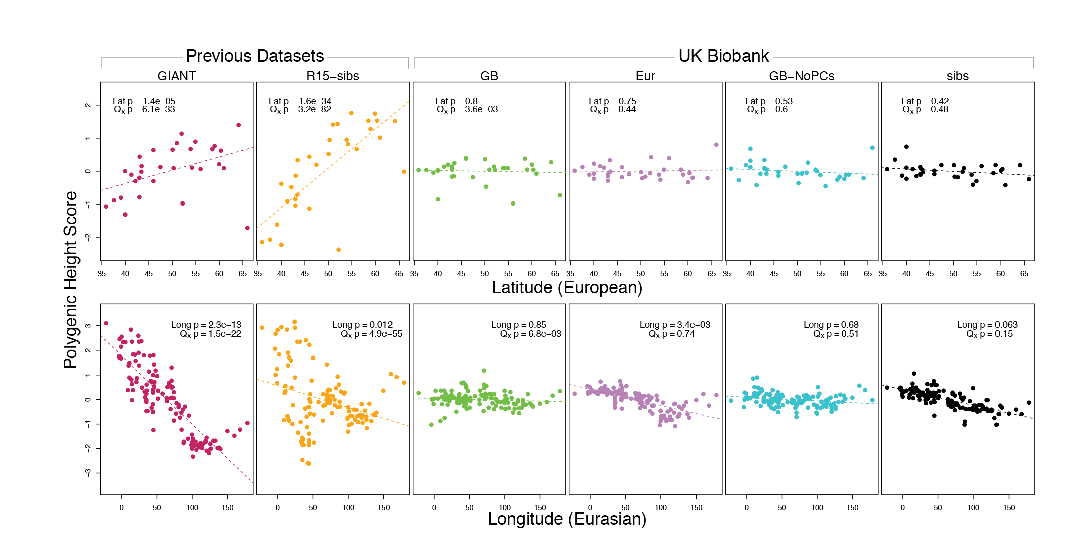
\includegraphics[width=\textwidth]{UK-biobank.eps}
  \end{center}
  
}

\myslide{
  \heading{Natural selection on height in humans}

  \noindent All data sets show real associations with height

  \noindent GIANT and R-15 fail to fully remove confounding variation
  along major geographic axes

  \noindent ``[W]hat once appeared an ironclad example of population
  genetic evidence for polygenic adaptation now lacks any strong
  support.''

}

\myslide{
  \heading{Extrapolating genomic predictions}

  \noindent Stabilizing selection for the same optimum phenotype in
  two genetically isolated populations

  \noindent Expectations

  \begin{itemize}

    \item Same selection: Same phenotypes

    \item Genetic isolation:

      \begin{itemize}

        \item No selection: Populations diverge
        
        \item With selection: \color{red}{\bf ?}

      \end{itemize}

    \end{itemize}

}

\myslide{
  \heading{Extrapolating genomic predictions}

  \begin{center}
    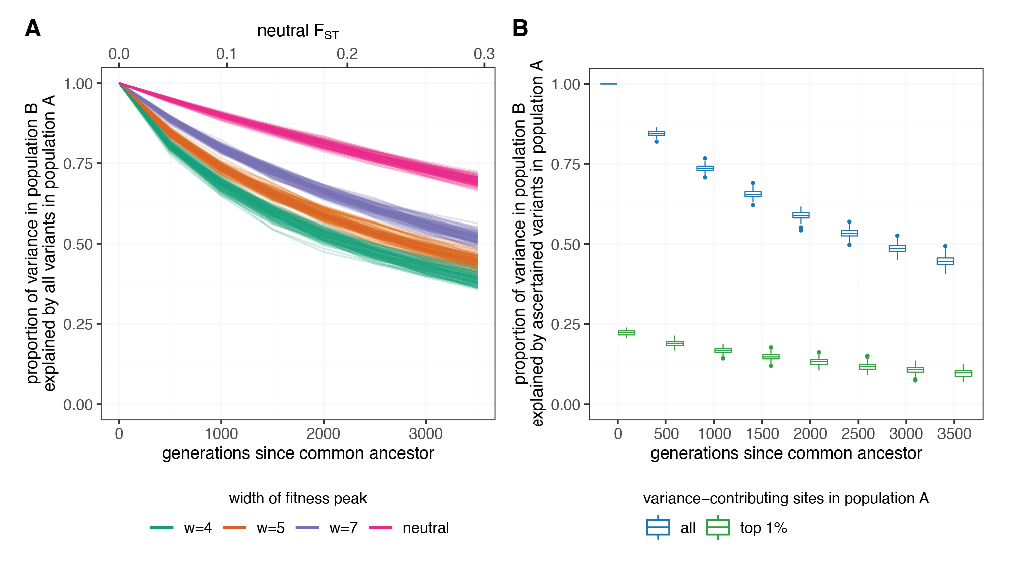
\includegraphics[width=\textwidth]{yair-coop-predictions.eps}
  \end{center}
  
}

\myslide{
  \heading{Genetic redundancy}

  \begin{center}
    \includegraphics[width=0.6\textwidth]{Nilsson-Ehle.eps}
  \end{center}
  
}

\myslide{
  \heading{Genetic redundancy: isolation by distance}

  \begin{center}
    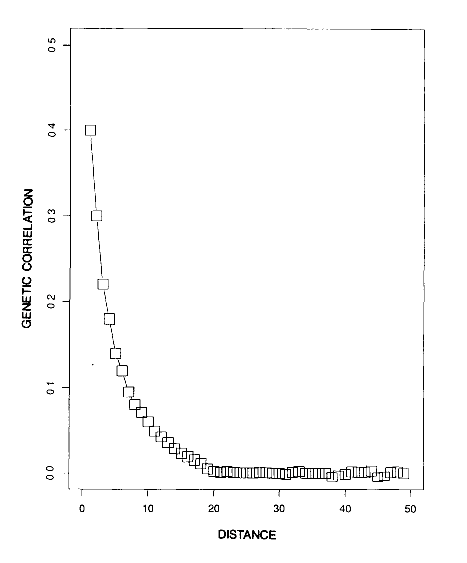
\includegraphics[height=0.8\textheight]{isolation-by-distance.eps}
  \end{center}
  
}

\myslide{
  \heading{Genetic redundancy: isolation by distance}

  \begin{itemize}

  \item Uniform selection for an intermediate genotype

  \item Many genotypes produce the same phenotype

  \item Individuals separated by a long distance evolve independently,
    even though selection produces the same phenotype

  \item Different genotypes produce the same phenotype in different
    parts of the population

  \item Genomic scores estimated in one part of the population won't
    extrapolate to a different part of the population

  \end{itemize}
}

\end{document}
